\documentclass{article}

\usepackage{color}
\usepackage[margin=1in]{geometry}
\usepackage{graphicx}
\usepackage{hyperref}
\usepackage{listings}

\definecolor{gray}{rgb}{0.5, 0.5, 0.5}
\definecolor{darkgreen}{rgb}{0, 0.6, 0}

\begin{document}
    \raggedright
    Homework 4 \break
    Christopher Seagraves
% % % % % % % % % % % % % % % % % % % % % % % % % % % % % % % % % % % % % % % % 

    \section*{Problem 1}
        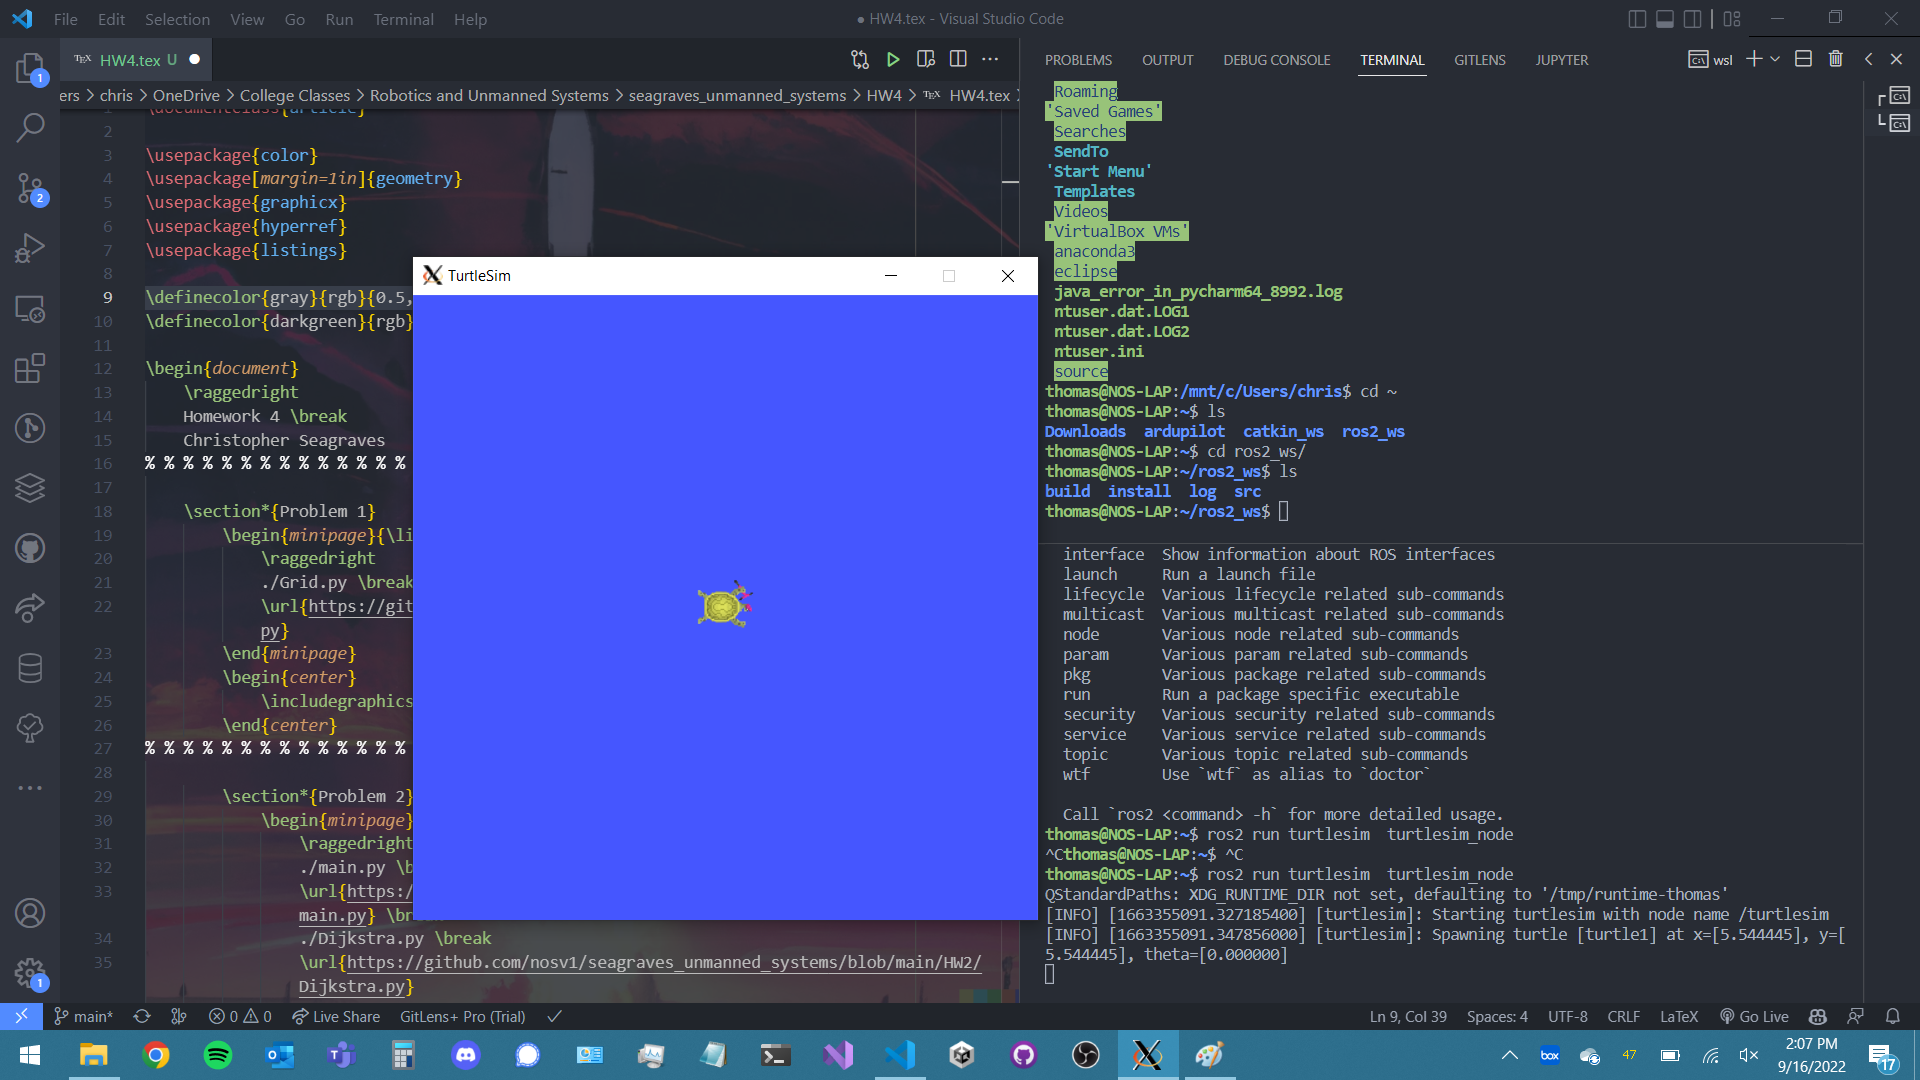
\includegraphics[width=\linewidth]{Problem 1 Turtlebot Simulator.png}
% % % % % % % % % % % % % % % % % % % % % % % % % % % % % % % % % % % % % % % %

    \section*{Problem 2}
        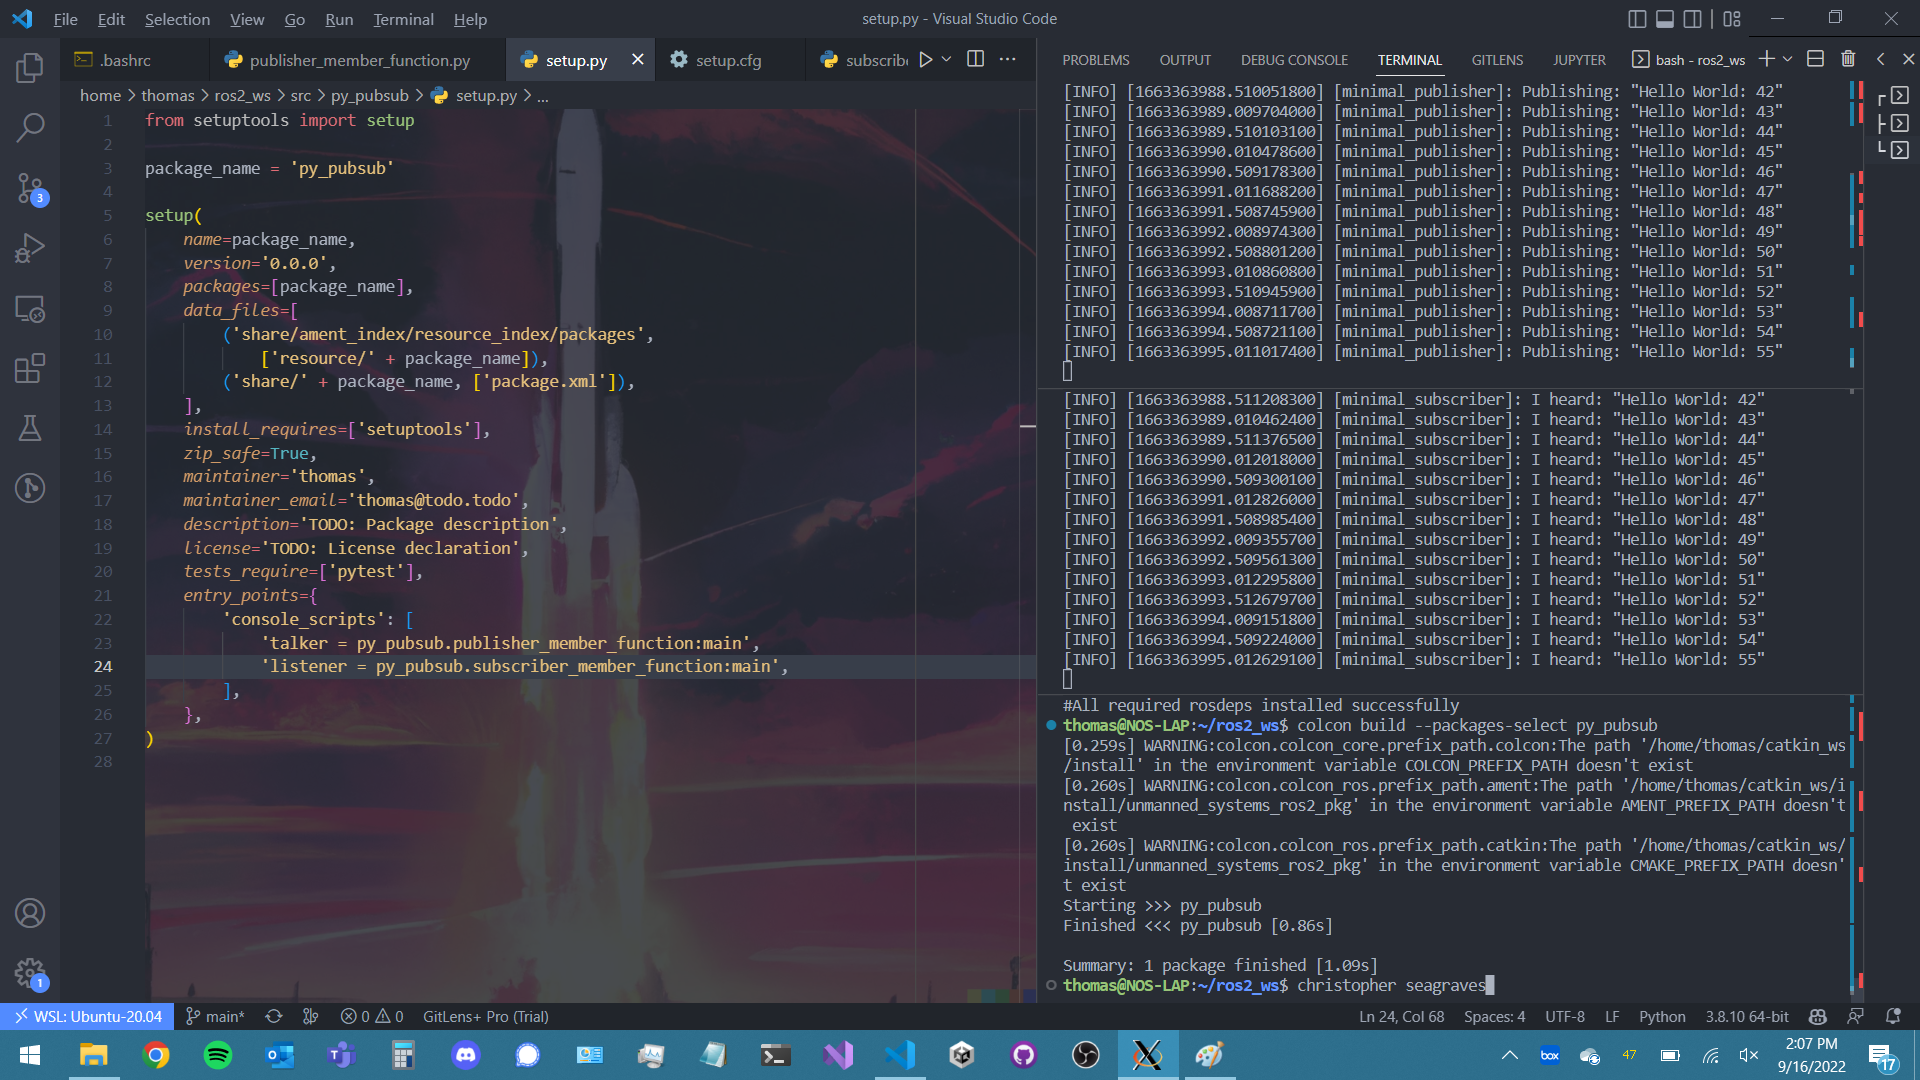
\includegraphics[width=\linewidth]{Problem 2 Publisher and Subscriber.png}
% % % % % % % % % % % % % % % % % % % % % % % % % % % % % % % % % % % % % % % %

    \section*{Problem 3}
        \raggedright
        command\_controller.py \break
        \url{https://github.com/nosv1/seagraves_unmanned_systems_pkg/blob/master/seagraves_unmanned_systems_pkg/command_controller.py} \break
        ./LogPlotter.py \break
        \url{https://github.com/nosv1/seagraves_unmanned_systems/blob/main/HW4/LogPlotter.py} \break
        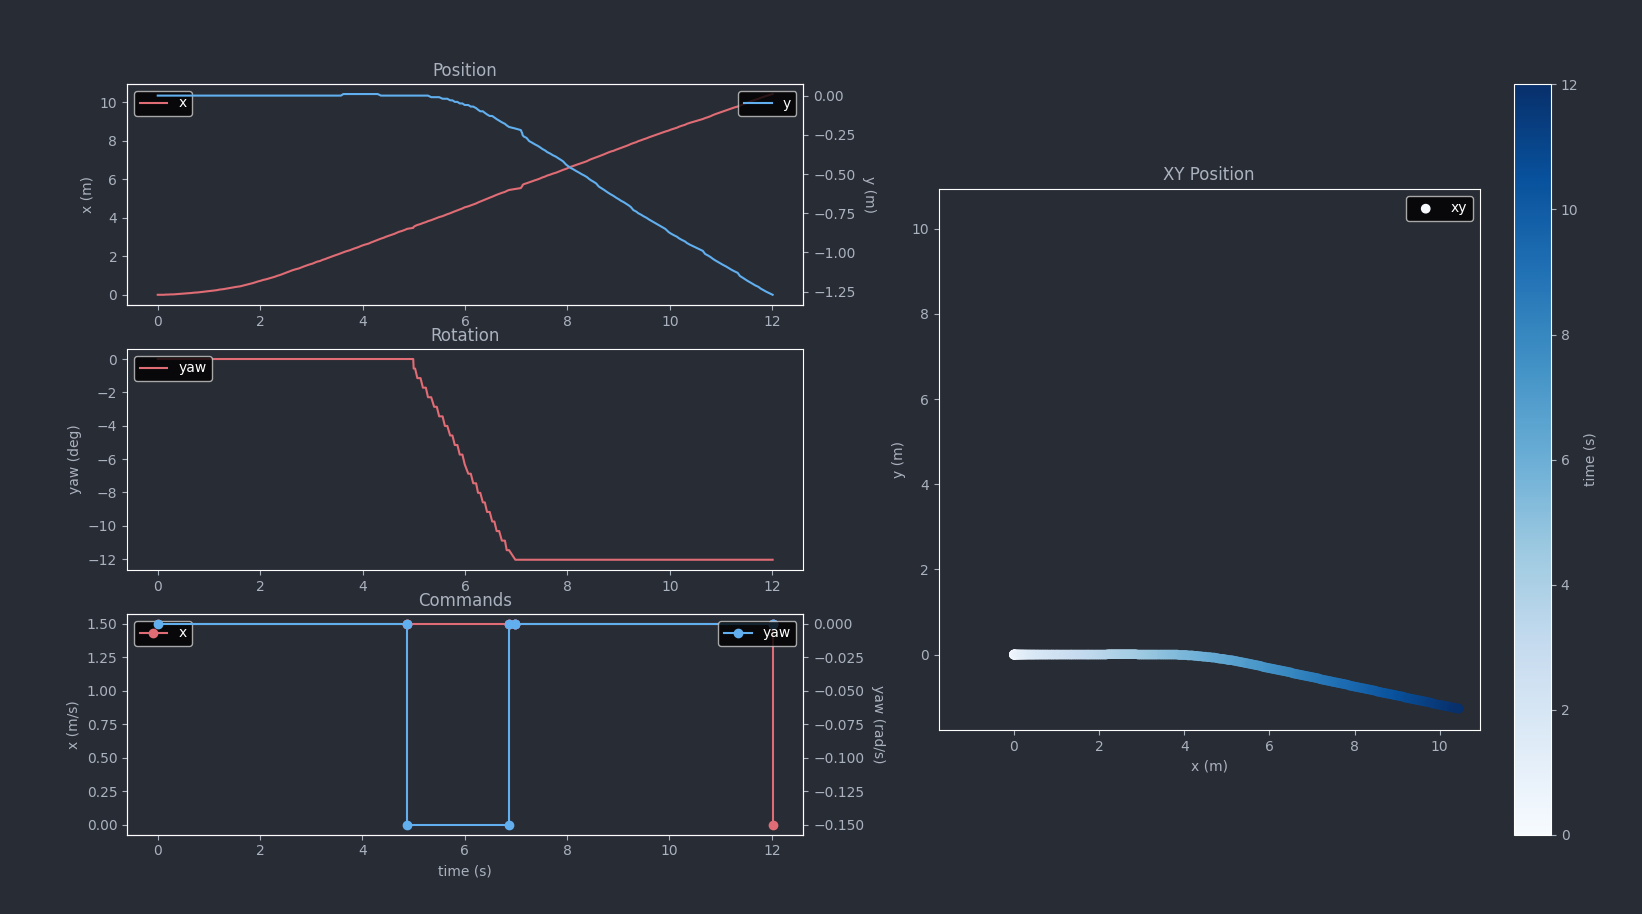
\includegraphics[width=\linewidth]{Problem 3 Telemetry.png}
    
    \section*{Problem 4}
        \raggedright
        Kp = 6.5, Ki = 0.0, Kd = 0.0 \break
        Rise time = 0.6 seconds \break
        Given Burger can turn at 2.84 rad/s (162.4 deg/s), it can complete a 90 degree turn in 0.55 seconds - about .05 seconds per 10 degrees - so the optimal rise time would be about 0.44 seconds.
        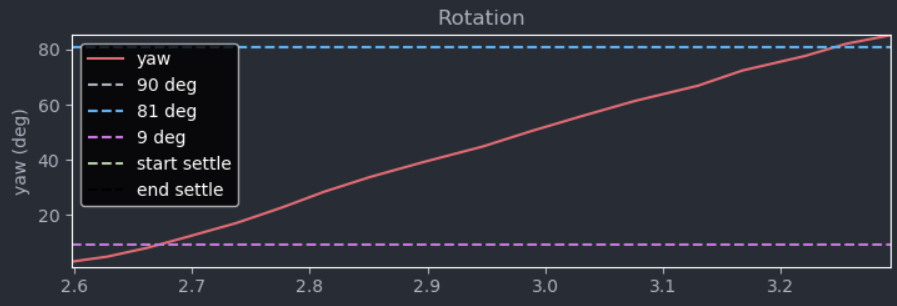
\includegraphics[width=\linewidth]{Problem 4 Rise Time.png} \break
        Settle time = 0.2 seconds \break
        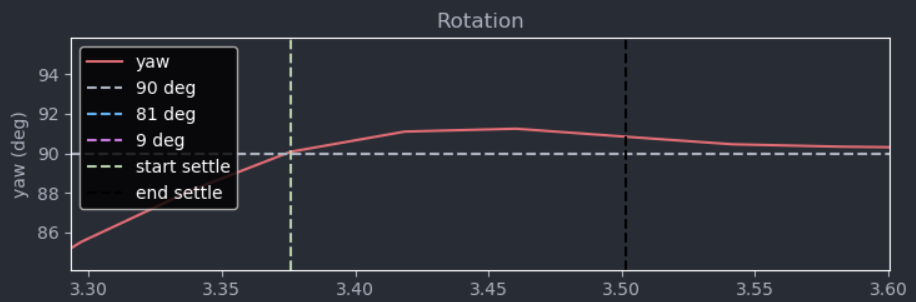
\includegraphics[width=\linewidth]{Problem 4 Settle Time.png} \break
        Percent overshoot = 1\% 1 - (91.2 / 90) \break
        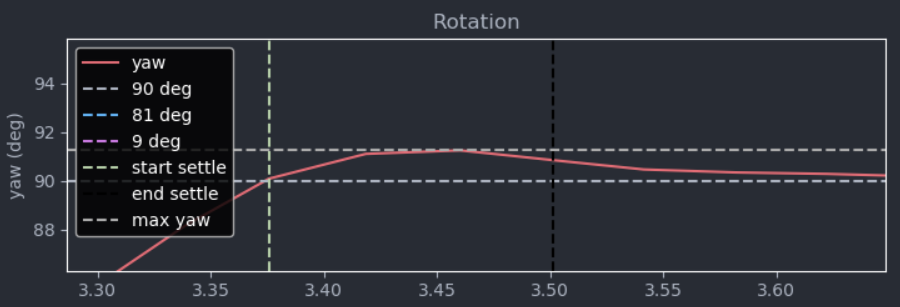
\includegraphics[width=\linewidth]{Problem 4 Percent Overshoot.png} \break
        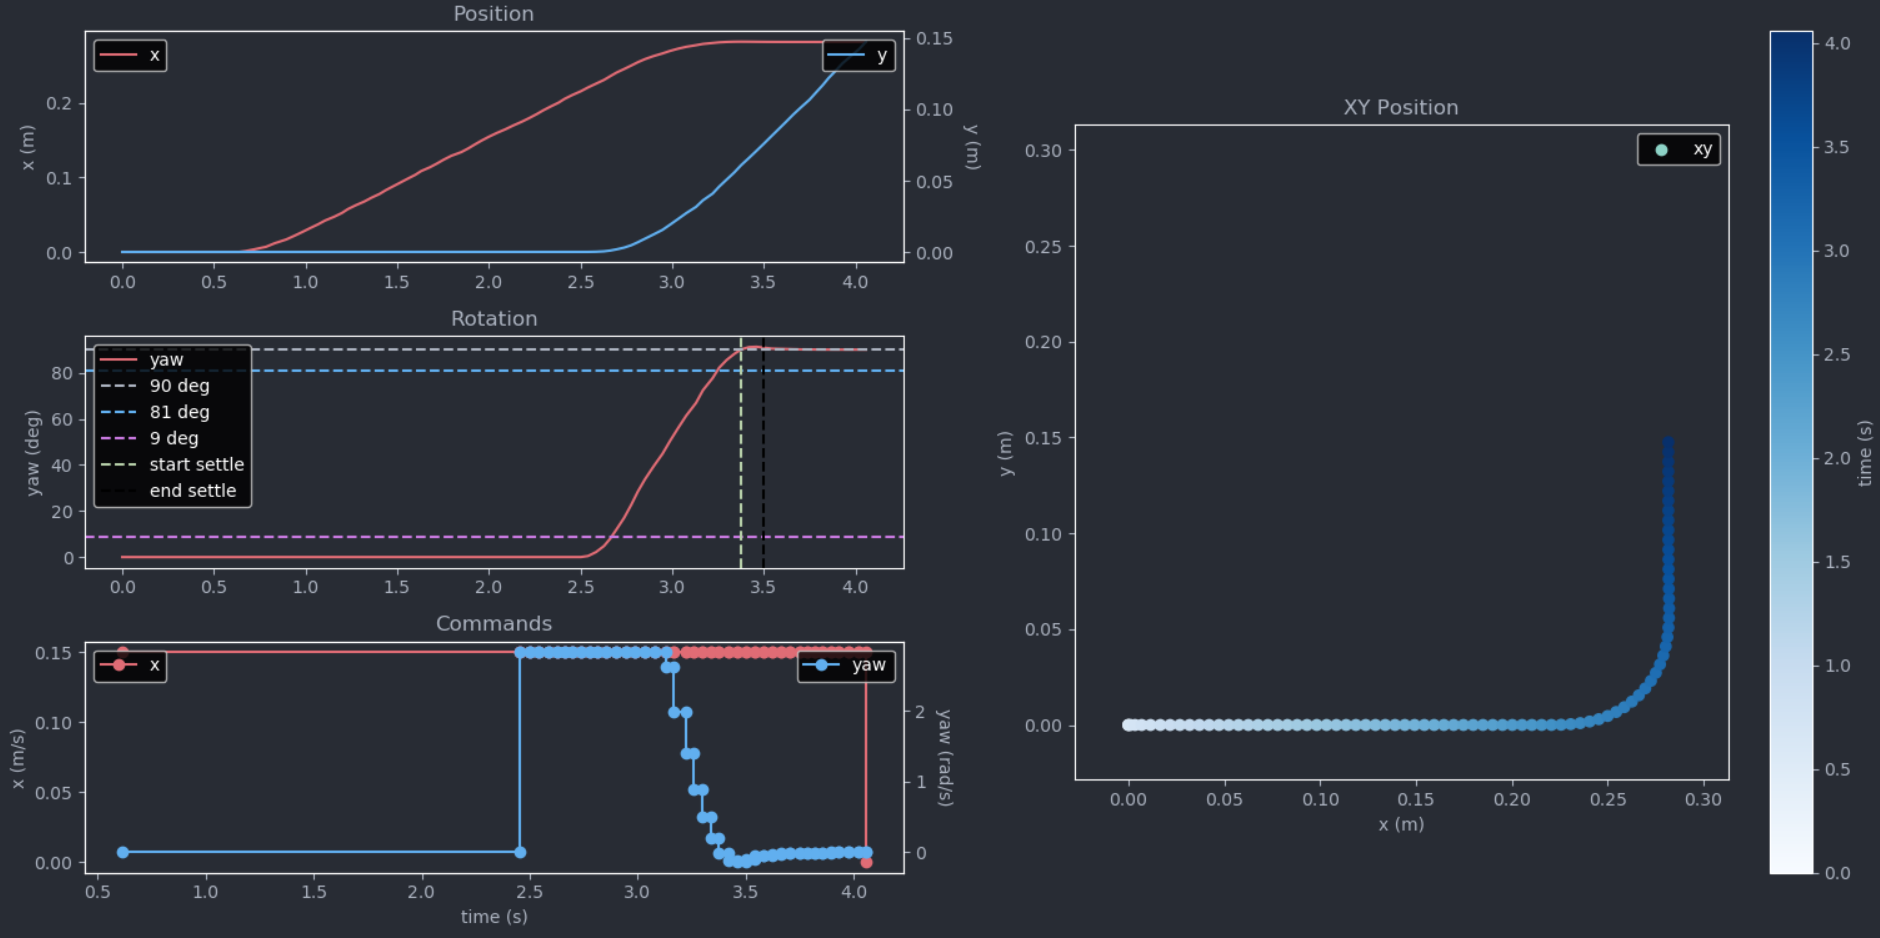
\includegraphics[width=\linewidth]{Problem 4 Telemetry.png}

    \section*{Problem 5}
        \raggedright
        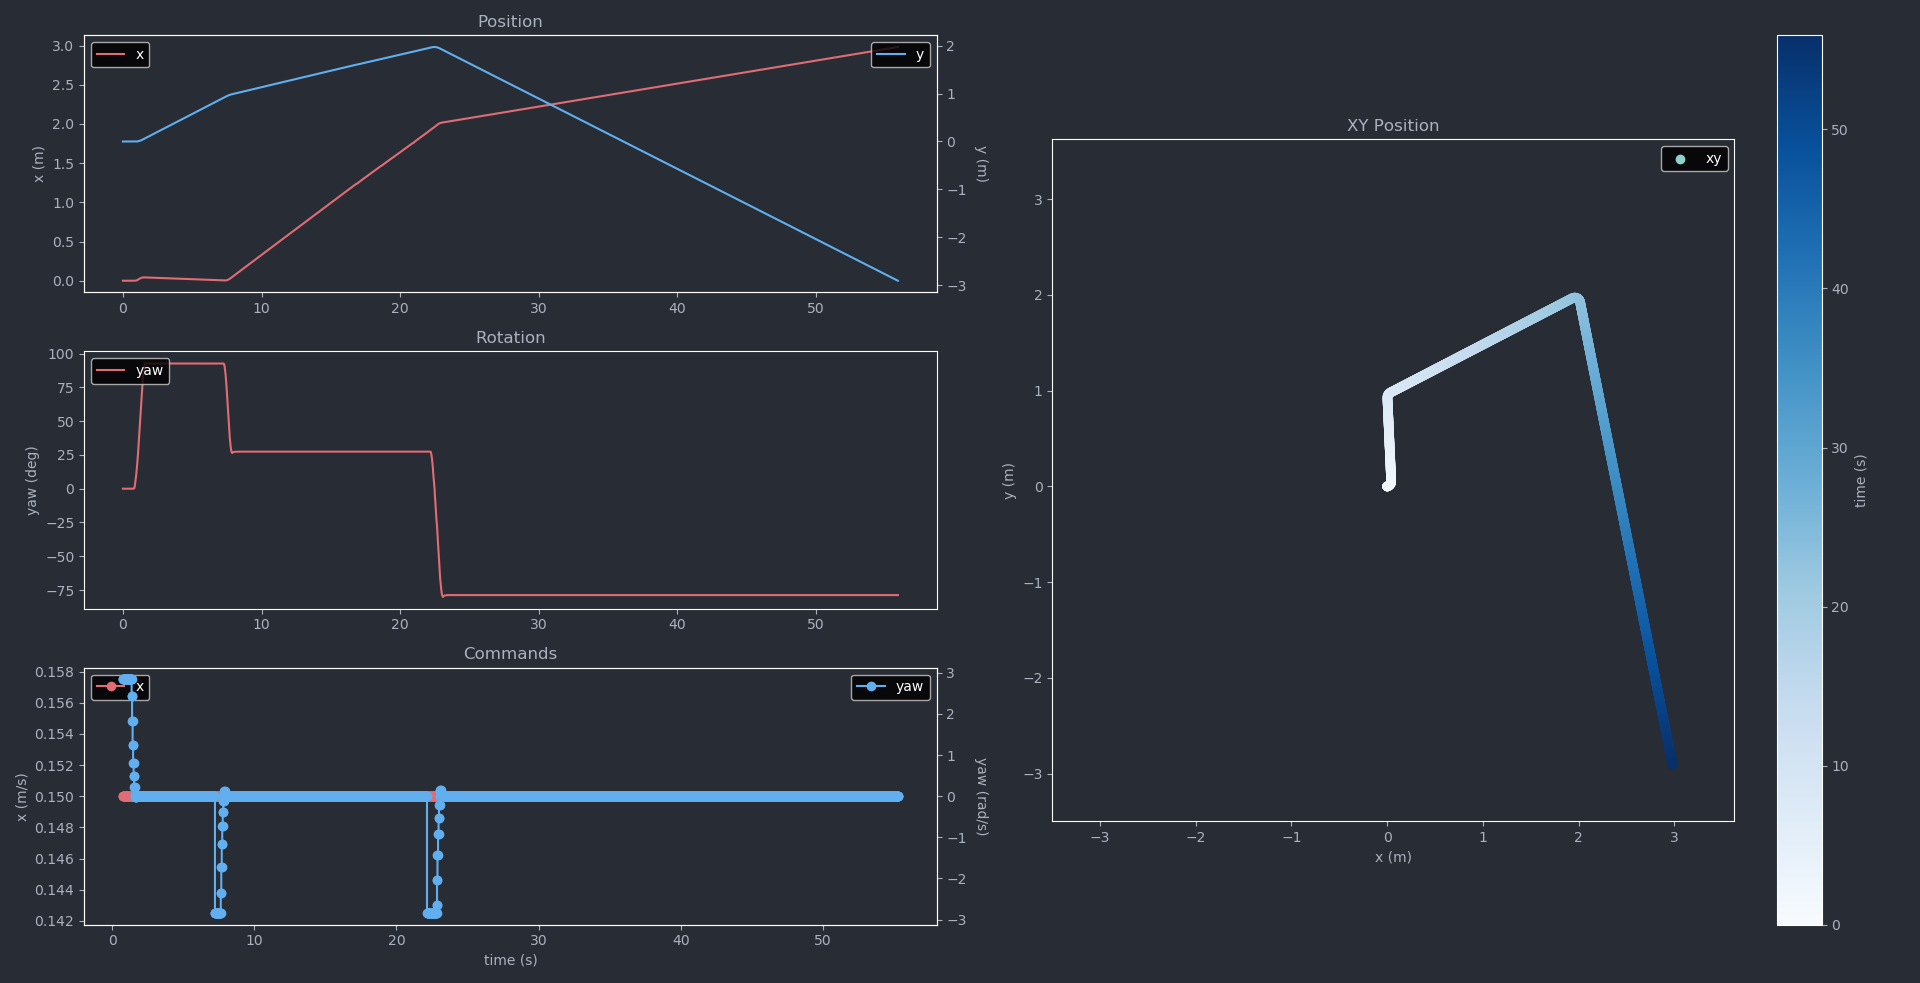
\includegraphics[width=\linewidth]{Problem 5 Telemetry.png}
% % % % % % % % % % % % % % % % % % % % % % % % % % % % % % % % % % % % % % % %

\end{document}